\todo{predelat na spravny format pdf}
\todo{zeptat se na odkazy u obrazku a odkazy u FANN a URHO3D}
\todo{vytvorit apendix}
\todo{ma byt intorduction chapter s cislem?}

\chapter{Introduction}
Magic has been a popular part of computer games since their beginning. In many games, magic has its own lore and laws that make it systematical. Great examples of a complexity of magical spells are games \emph{Magicka} and \emph{Magicka 2}, where player casts spells by combining eight elements \ref{fig:magicka}. For example, using only earth element results in a rock thrown at the enemy, but adding fire will create a classic fireball.
\begin{figure}[!htb]
  \centering
  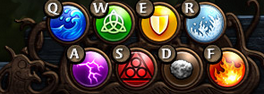
\includegraphics[width=0.5\textwidth]{ext/magicka.png}
  \caption{\emph{Magicka} spell interface}
  \label{fig:magicka}
\end{figure}

In books and movies, we can see wizards performing complicated hand gestures, or drawing on the floor some complex shapes. However, in games it is quite easy to do magic, since players often push a few buttons for even the strongest spells. This spoils the feeling of magic as something extraordinary and secret. We would like to allow developers to take a different approach, which requires players focus and concentration, as well as possible cooperation in spell casting.

While a majority of games binds spells to buttons, there are several games that used pattern recognition in their spell system. However, these systems recognized only simple gestures or patterns. Our goal is to make a more robust recognition system, that allows players to draw complex patterns.

\section{Pattern recognition in current games}

Since symbols and gestures are an integral part of the magic, there were many attempts to bring them into video game environment. \citet{gameMagic} provides a classification of gestural systems into three categories, which are overlapping, as sometimes combination of these approaches can be used. The following categories and facts are taken from \citet{gameMagic}.

\begin{description}
\item[Alternative controllers]
One such category are systems that utilize alternative controllers to mouse and keyboard, such as Kinect. Recent game from this category is \emph{Fable: The Journey}, where player casts spells by moving his hands. For example, push spell is cast by pushing into the air. Patterns made by the player are then recognized using Kinect technology. While moves are simple in nature, such as waving sideways or back and forth, both hands at the same time can be used, resulting in quite complex gestures.

\item[Restricted drawing forms]
Another technique used in several games is to let player draw into a predefined grid, or through predefined points. Both \emph{Castlevania: Dawn of Sorrow} and \emph{Deep Labyrinth} take advantage of an Nintendo DS drawing interface that allows players to draw magic signs. 
In \emph{Castlevania}, players draw signs by connecting glowing points in a circle in out-of-combat situations, as seen in \cref{fig:castlevania}. \emph{Deep Labyrinth} introduces special casting interface as well, consisting of 3x3 sized grid, where player connects dots. These approaches take away part of the freedom, but they make recognition algorithms much easier, e.g. by tracing only the order of points and selecting the right spell.

\begin{figure}
\centering
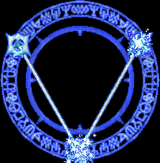
\includegraphics[width=.3\linewidth]{ext/castlevania.png}
\quad
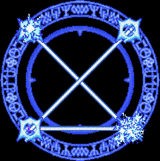
\includegraphics[width=.3\linewidth]{ext/castlevania2.png}
\caption{\emph{Castlevania: Dawn of Sorrow} spell interface \XX{(image taken from ?)}}
\label{fig:castlevania} %label se vaze na caption a musi bejt az po nem
\end{figure}

\item[Free-hand drawing]
To this category belong the examples that are most similar to our goal. One of the first games to integrate some form of pattern recognition of drawn shapes is \emph{Black \& White}, where the player takes a role of the god. Using a mouse, players are able to cast miracles by drawing a specific pattern onto the ground \ref{fig:blackwhite}. The player can draw anything anywhere on the ground, and its up to the game algorithm to recognize if it matches some of the miracle patterns. Alternatively, the player also cast miracle by clicking on a button, presumably because a lot of players had trouble drawing the miracles. 
A similar approach to recognition of player drawn spells and their recognition is used in \emph{Arx Fatalis}. Players are drawing symbols into the air with a mouse and the sequence of symbols represents some spell. While casting, game encoded the mouse moves into characters in 8-directions precision, each direction representing some letter. After player finished their spell, a Levenshtein distance was calculated from each predefined spell sequence to the user's created sequence and the candidate with the lowest Levenshtein cost was returned as a matching spell.

\begin{figure}
\centering
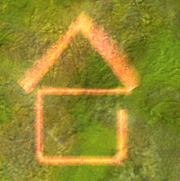
\includegraphics[width=.3\linewidth]{ext/gestureteleport.png}
\quad
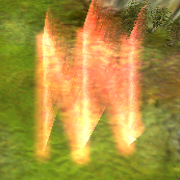
\includegraphics[width=.3\linewidth]{ext/gesturefireball.png}
\caption{\emph{Black \& White} teleport and fireball gestures}
\label{fig:blackwhite}
\end{figure}

\end{description}

\section{Goals}

We would like to allow players to draw complex spells. Instead of a sequence of symbols recorded over time, players could draw symbols arranged in a shape of another symbol, or embed one symbol in another. We also want our approach to be applicable in multi-player environments, where new situations can occur, such as multiple players drawing one spell. We don't want to introduce the aiding structures as in \cref{fig:castlevania} since they require and order in which they are passed and force the player to draw in a certain way or direction. They are also not very suitable for a multi-player environment since they can't handle multiple people drawing at the same time.

For the purpose of this work, we specify the following requirements that we have on our recognition system.
\begin{description}

\item [Durability against shape deformations]
Since we want to recognize hand-drawn shapes, our system has to be prepared for human-like imprecise drawing, especially when drawing with a mouse. However, defining what is deformed within some boundaries and should be recognized, and what is too deformed, is a difficult task.

\item [Extensibility]
We would like to offer an easy-to-use library that can be applied to other projects. For this purposes, we would like to let users define their own shapes that should be recognized. Our framework will offer interfaces for both preparing their own shapes and using them in the pattern recognition.

\item [Performance]
Our system should be applicable in demanding video games environment, prepared for the possibility of many players drawing their spells. To achieve this, we require fast recognition technique as well as usability in a parallel environment. 

\item [Recognition of embedded shapes]
To allow players cast complex spells, we need to give them an ability to somehow encode multiple symbols in one spell. One possible way to do it are shape embeddings. Each defined shape can contain several areas, where other shapes might occur. These areas are then processed in our recognition system and classified.

\item [Recognition of shape conglomerations]
For the purpose of this work, we consider shape conglomeration a group of shapes from the same shape class e.g. circle, arranged such that the whole conglomeration forms another shape. We can also look at it as taking the curves of the shape, sampling them uniformly, and then replacing all the samples with the pattern shape.

\end{description}

\begin{figure}
\centering
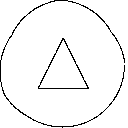
\includegraphics[width=.3\linewidth]{ext/images/embedd.png}
\quad
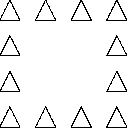
\includegraphics[width=.3\linewidth]{ext/images/comp.png}
\quad
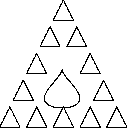
\includegraphics[width=.3\linewidth]{ext/images/comp_and_embed.png}

\vspace{1cm}

\centering
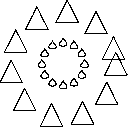
\includegraphics[width=.3\linewidth]{ext/images/comp_in_comp.png}
\quad
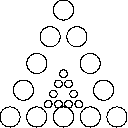
\includegraphics[width=.3\linewidth]{ext/images/comp_in_comp2.png}
\quad
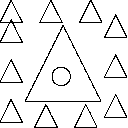
\includegraphics[width=.3\linewidth]{ext/images/triple.png}
\caption{In the figure, embedded positions are always in the middle of the shape. From left to right: circle with embedded triangle; square composed of triangle; triangle composed of triangle, with water drop embedded; circle composed of triangles, with embedded circle composed of water drop; triangle composed of circle, with embedded triangle composed of circle; square composed of triangle, with embedded triangle, with embedded circle in the triangle}
\label{fig:examples} 
\end{figure}

\subsection{Approach}
To achieve our goals, we divide the work into several steps. First, we have reviewed approaches and algorithms commonly used to solve pattern recognition problem. We have closely examined three algorithms, namely the \emph{Normalized cross-correlation},\emph{Shape matching and object recognition using shape contexts} and \emph{Matching of Shapes Using Dynamic Programming}. Then we have described \emph{Artificial neural networks} and explain, how to apply them to pattern recognition. In the \cref{ch:impl}, we have described our algorithm, which is based on the neural networks. We also developed a simple game prototype, to demonstrate the usage of our recognition system. Finally, we perform measurements of the performance of our algorithm, with respect to recognition success rate and speed.

In the appendix, we have described the interface of our algorithm and how to use it in another project. We have also provided a guide for the game.